\chapter{Algoritmo de Diversidad basado en Dominancia} % Main chapter title

\label{Chapter3}

\section{Introducción}

Los algoritmos evolutivos (EA) son considerados como uno de los enfoques más prometedores en distintos problemas de optimización, tanto en dominios continuos como en discretos.
%
Además, se han vuelto bastante populares en las últimas décadas en parte por el incremento de las capacidades de cómputo.
%
Por lo tanto los EAs son utilizados ampliamente en diversas áreas de estudio y aplicaciones del mundo real.
%

%

Se ha demostrado que el rendimiento de un algoritmo evolutivo es afectado por falta de soluciones diversas.
%
Así, los algoritmos diagnosticados con problemas de diversidad pueden guiar el proceso de búsqueda a regiones complicadas, por lo tanto todos los miembros de la población son situados en una parte reducida del espacio de búsqueda, siendo distinta de la región de soluciones óptimas, además los componentes del algoritmo no permiten escapar de estas regiones, en el ámbito mono-objetivo esto es un inconveniente y es definido como convergencia prematura (\cite{Joel:Crepinsek}).
%
Además, se ha demostrado que un algoritmo evolutivo el cual proporciona un balance entre intensificación y exploración puede generar resultados de alta calidad e inclusive mejores que el promedio de algoritmos.
%
Por otra parte si la población es muy diversa, entonces la fase de explotación puede ser afectada, en consecuencia la convergencia del algortimo es muy lenta, proporcionando soluciones muy lejanas de la región óptima.
%
Por lo tanto \citeauthor{Joel:mahfoud1995niching} en \citetitle{Joel:mahfoud1995niching} define el concepto de diversidad útil como las cantidades de diversdad que proporcionan soluciones de calidad.
%Además el efecto que tiene la diversidad por parte de las soluciones en un algortimo evolutivo es evidente en la calidad de las soluciones, como es expliaco por ... en REF.
%

En la búsqueda de preservar un balance entre exploración e intensificación por parte del proceso evolutivo, se han desarrollado algoritmos mediante distintas estrategias, de esta forma se desea evitar el incoveniente de la convergencia prematura, los principales mecanismos utilizados son operadores de mutación disruptivos, tamaño de población variada, esquemas de reinicio, emparejamiento especial de padres (\cite{Joel:MOEAD_AMS}), modelos explícitos de seleccion (\cite{Joel:MULTI_DYNAMIC}), entre otros.
%
Sin embargo, no siempre se entiende plenamente la forma en que la exploración y la explotación se promueven en un EA, y dependen de una variante muy específica como parte de la estrategia implementada.
%
Por ejemplo, mientras en algunos esquemas el operador de mutación se encarga de promover la exploración (\cite{Joel:herrera2003fuzzy, Joel:CHC}), en otros casos esta tarea es asignada al operador de cruce (\cite{Joel:sivanandam2007introduction}). 


Aunque este trabajo se enfoca en la optimización multi-objetivo, las estrategias aquí presentadas pueden ser implementadas en el ámbito mono-objetivo sin cambios significativos.
%
%%%Se explican las secciones de este capítulo.

Inicialmente se mencionan algunas de las estrategias usadas para administrar la diversidad en el optmización mono-objetivo y multi-objetivo.
%
Posteriormente se explica el algoritmo propuesto en el ámbito multi-objetivo, considerado como el primer algoritmo basado en dominancia que administra la diversidad en las variables de decisión de forma explícita.
%
%
Adicionalmente se realiza una análisis de los beneficios y las desventajas del algoritmo propuesto, así mismo dando importancia a la diversidad en el espacio objetivo se presenta la fase de reemplazo que conforma parte del algoritmo VSD-MOEA y además se explica una simulación de los pasos involucrados en la fase de remplazo.
%
Por otra parte se propone la distancia de mejoría que está basada en el indicador IGD+, la cual es considerada como débilmente \textit{Pareto Compliance}.
%
Al final se muestra una simulación del VSD-MOEA junto al estado del arte en la problema de prueba WFG5 cuya principal característica es su transformación con propiedades deceptivas.

\section{Diversidad en el espacio de las variables en MOEAs}

En optimización estocástica, específicamente en el caso mono-objetivo, se ha desarrollado una variedad de algoritmos evolutivos con el propósito de tratar aspectos relacionados con la falta de diversidad, específicamente la convegencia prematura (\cite{Joel:Crepinsek}).
%
Algunos de los algoritmos populares que están relacionados con temas de diversidad son Saw-Tooth (\cite{Joel:SAWTOOTH}), CHC (\cite{Joel:CHC}) y Multi-Dynamic (\cite{Joel:MULTI_DYNAMIC}).
%
Este último relaciona el manejo de diversidad en el espacio de las variables con el criterio de paro establecido. % \cite{Joel:segura2016improving}.
%
De esta forma, y dependiendo del criterio de paro, en las fases iniciales se promueve un mayor nivel de exploración y conforme van transcurriendo las generaciones se realiza un cambio gradual para obtener un mayor nivel de intensificación.
%
Este control se puede realizar desde distintos enfoques, y se ha visto experimentalmente que actuar sobre varias fases puede ser beneficioso (\cite{Joel:ANovelDiversityBasedEAForTheTSP}).
%
Este tipo de métodos se han vuelto exitosos en optimización mono-objetivo, proporcionando el desarrollo de optimizadores que actualmente han encontrado los mejores resultados en varios problemas conocidos, como es el problema de ordenación lineal, el problema de asignación de frecuencias \citetitle{Joel:Dynamic_FAP}, el problema del Sudoku \citetitle{Joel:Dynamic_Sudoku}, el problema del agente viajero \citetitle{Joel:ANovelDiversityBasedEAForTheTSP}, entre otros.
%


En optimización multi-objetivo es posible encontrar los mismos inconvenientes que en problemas mono-objetivo, además al considerar varios objetivos que usualmente están en conflicto es necesario mantener soluciones diversas.
%
Así, un problema multi-objetivo está compuesto por dos espacios, el primero consiste en el espacio de las variables y sus respectivas imagenes conforman el espacio objetivo.
%
Además, no existe una correspondencia directa entre la diversidad de los dos espacios (\cite{shir2009enhancing}), esto quiere decir que un grado determinado de diversidad en el espacio objetivo no implica que siempre existirá un grado determinado de diversidad en el espacio de las variables.

% 
En todos los problemas multi-objetivo no existe una relación identica entre ambos espacios, debido a esto los MOEAs están diseñados principalmente para mantener diversidad en el espacio objetivo, perdiendo la influencia directa que existe por parte de la diversidad en espacio de las variables.

%
Actualmente ya existen varios trabajos que proporcionan relevancia a la diversidad en el espacio de las variables. % \citetitle{Joel:GECCO17}.
%
Una estrategia popular consiste en aplicar restricciones para realizar el emparejamiento de los individuos (\cite{Joel:MOEAD_AMS}), en base a varios estudios presentados en \citetitle{Joel:STUDY_MATTING_RESTRICTION} por \citeauthor{Joel:STUDY_MATTING_RESTRICTION}, donde se define una restricción de emparejamiento específicamente con soluciones cercanas o similiares en el espacio de las variables, debido a que emparejar dos individuos alejados tiende a generar individuos distantes y no útiles en el espacio de búsqueda.
%
Otra alternativa consiste en implementar esquemas de reinicios (\cite{ joel:jaeggi2008development, Joel:Improved_Multiobjective_Diversity_Control_Oriented_Genetic_Algorithm}).
%
Sin embargo en el caso multi-objetivo no se ha establecido una propuesta en donde la diversidad sea administrada de forma explícita y que dependa del criterio de paro.
%


En base al estudio de diversidad realizado por \citeauthor{Joel:GECCO17} en \citetitle{Joel:GECCO17} se ha comprobado que los MOEAs poseen problemas de diversidad.
%
Específicamente en este capítulo se utiliza el mismo principio que en \citeauthor{Joel:MULTI_DYNAMIC}, que está diseñado especialmente para problemas de un solo objetivo y administra la diversidad en el espacio de las variables de forma explícita. 

\section{Trabajos relacionados}

A través de las últimas décadas se han presentado varios trabajos de tipo multi-objetivo que están relacionados con promover soluciones diversas en el espacio de las variables, así los primeros trabajos surgieron con el propósito de resolver funciones objetivo de tipo multi-modal (\cite{preuss2006pareto}).
%In the MOEAs literature several analyzes of diversity in decision space are presented, in particular some of them are oriented to solve multi-modal objective functions \cite{preuss2006pareto}.
%
En especial, esta categoría de algoritmos pueden ser de interés en problemas de aplicación real, ya que es necesario proporcionar soluciones bien distribuidas en el espacio de decisión (\cite{deb2005omni, rudolph2007capabilities}).
%In special, they are considered based in real applications where high diversity solutions in the decision space can be of interest for decision makers \cite{deb2005omni, rudolph2007capabilities}.
%
En base a las estrategias utilizadas en un sólo objetivo, se han propuesto distintas técnicas de nichos en el campo de optimización multi-objetivo.
%As in single-objective diversity techniques some niching techniques has been already used in the multi-objective optimization field. 
%
De hecho uno de los primeros MOEAs que introducen este tipo de técnicas es el NPGA (Nicho Preto Genetic Algorithm - \cite{Joel:NPGA}).
%In fact one of the first MOEAs that introduces niche technique is the NPGA (Nicho Pareto Genetic Algorithm) . 
%
Este algoritmo es una variante del método de nichos con aptitud compartida (\textit{fitness sharing niching method}).
%This algorithm was a variant of the fitness sharing niching method.  

%
Posteriormente, \citeauthor{toffolo2003genetic} en el \citeyear{toffolo2003genetic} propusieron otro algoritmo para obtener soluciones diversas tanto en el espacio de las variables como en el espacio objetivo conocido como GDEA.
%Another MOEA designed to attain a good diversity in decision as well as in objective space was the GDEA, introduced by Toffolo and Benini in 2003 \cite{toffolo2003genetic} .
%
Este algoritmo implementa dos criterios de selección, el primero por medio de una ordenación de soluciones no dominadas y el segundo consiste en una métrica para la diversidad en el espacio de la variables.
%GDEA invoked two selection criteria, non-dominated sorting as the primary one and a metric for decision space diversity as secondary one.
%

En el \citeyear{deb2005omni}, \citeauthor{deb2005omni} propusieron el ``Omni-optimized'' considerado como una generalización del NSGA-II, en este algoritmo se incorpora la diversidad en los dos espacios, además se propone un nuevo criterio de selección y se aplica la definición de dominancia-$\epsilon$.
%Thereafter, a popular diversity approach implemented was the Omni-Optimizer in 2005 \cite{deb2005omni}, which is a generalization of the NSGA-II where is considered the diversity in the decision space.
%
Sin embargo, en el proceso de selección únicamente se considera la diversidad de un espacio por cada generación.
%Its selection is performed with a changing secondary selection criterion, orienting either the decision or objective space diversity in each generation.
%

En el \citeyear{chan2005evolutionary}, \citeauthor{chan2005evolutionary} propusieron dos operadores de selección, para fomentar la diversidad en cada uno de los espacios.
%
Particularmente, se implementaron estos operadores en los algoritmos KP1 y KP2.
%
Así, en cada generación son implementados dos criterios para medir la diversidad de las soluciones en los espacios correspondientes.
%Similarly, in 2005 Chan and Ray \cite{chan2005evolutionary} suggested using two selection operators in MOEAs; one encourages the diversity in the objective space and the other does so in the decision space. They implemented KP1 and KP2, two algorithms using these two selection operators.
%
%Additionally, a MOEA approach designed for maintain diversity in both spaces is the KP1 proposed by Chan and Ray \cite{chan2005evolutionary}.
%
%Here, two criteria to measure the diversity solutions in the corresponding spaces are defined and applied in each generation.
%
Estos son el hipervolumen de cada individuo para el espacio objetivo y un conteo de los vecinos para el espacio de las variables.
%These are the dominated hypervolume of each individual for the objective space and a neighborhood counting approach for the decision approach.
%

En el 2009, \citeauthor{shir2009enhancing} propusieron una variante del NSGA-II conocido como ``NSGA-II-agg'', donde se realiza la agregación de la diversidad presentada en los dos espacios, principalmente en este trabajo se propone el Niching-CMA.
%
%In 2009, a variant of the NSGA-II denoted as NSGA-II-agg was presented by Shir et al. \cite{shir2009enhancing}, which considers an aggregated space in the crowding calculations, also in this work is proposed the Niching-CMA.
%

Uno de los primeros algoritmos que considera la diversidad y es basado en indicadores es denominado como el DIVA (\textit{Diversity Integrating Hypervolume-based Search Algorithm}) propuesto en el \citeyear{ulrich2010integrating} por \citeauthor{ulrich2010integrating}, donde se combina la diversidad en el espacio de la variables y el indicador del hipervolumen, para realizar esto se modifica la métrica del hipervolúmen conformado por la suma de particiones en el espacio objetivo, donde cada partición es multiplicada por un factor que corresponde a la diversidad en el espacio de las variables, sin embargo esta modificación del hipervolumen aún se considera como Pareto \textit{compliant}.
%
Un aspecto interesante de este algoritmo es que en el espacio de las variables se consideran vecindades en base a hiper-rectángulos.
%In recent years, the DIVA (Diversity Integrating Hypervolume-based search Algorithm) was proposed in 2010 by Ulrich et al. \cite{ulrich2010integrating}, this combines the decision space diversity and hypervolume indicator values. 

Por otra parte, siendo parte de la familia de EDAs (Algoritmos de Estimación de Distribución) se encuentra el MMEDA propuesto por \citeauthor{zhou2009approximating} en el \citeyear{zhou2009approximating}, este implementa una fase de modelación donde la población es agrupada en base al espacio objetivo y posteriormente se genera un modelo probabilistico para la distribución de soluciones óptimas en el espacio de las variables.
%
Este modelo puede promover la diversidad en los dos espacios.

%
%Another style of EA based in a estimation distribution algorithm MMEDA \cite{zhou2009approximating} proposed in 2009 implements a modeling phase where the population is clustered based in the objective space and it generates a probabilistic model for the distribution of the Pareto-optimal solutions in the decision space.
%
%Such a model could promote the population diversity in both spaces. 
%

Actualmente, se han presentado varios trabajos que corresponden a las variables de decisión, algunos están orientados hacia la escalabilidad de las variables e implementan procesos de aprendizaje para capturar dependencias como es el algoritmo \citetitle{ma2016multiobjective} propuesto por \citeauthor{ma2016multiobjective} en el \citeyear{ma2016multiobjective}.

%Thereafter, a research line has been increasing that is oriented in the scalability of the decision space, e.g based in interdependence detecting techniques \cite{ma2016multiobjective} in 2016. 
%
%Despite the fact that are present some MOEAs oriented in diversity space, does not exist a MOEA which depend of the criteria stop and provides well disperse individuals in both spaces and improves the popular state-of-art algorithms.

\section{Propuesta}

Los algoritmos basados en dominancia son considerados como una categoría fundamental del ámbito multi-objetivo, en particular esta propuesta se enfoca en el concepto de dominancia, esta familia de algoritmos han estado creciendo las últimas dos décadas, principalmente los algoritmos basado en dominancia son implementados en problemas de dos y tres objetivos, ya que existen problemas de convergencia al frente de Pareto al incrementar el número de objetivos (\cite{Joel:Coello, Joel:Kalyanmoy}).
%
Particularmente, en este MOEA se establece una fase especial de reemplazo, donde se define un procedimiento sencillo para administrar la diversidad en las variables y en los objetivos, posteriormente se propone una distancia de mejoría en el procedimiento para administrar la diversidad en el espacio objetivo de forma más adecuada, esta distancia está relacionada con el indicador del hipervolúmen. 

%
El procedimiento principal de la propuesta se observa en el algoritmo \ref{alg:VSD_MOEA}, donde primeramente se realiza la inicialización de la población $P_0$ con $N$ individuos y sus respectivas evaluaciones en las líneas \ref{alg:VSD_MOEA_Linea1} y \ref{alg:VSD_MOEA_Linea2}.
%
En este algoritmo el conjunto $P$ representa a los individuos padres y $Q$ a los individuos hijo.
%

Inicialmente el conjunto de individuos hijo $Q_0$ esta vacío, pero en cada generación $t$ del ciclo principal, los individuos hijo $Q_{t}$ corresponden a los nuevos individuos.
%
Así, como es usual de un algoritmo evolutivo, se aplica la \textbf{Selección} basada en el torneo binario en la línea \ref{alg:VSD_MOEA_Seleccion}.
%
Posteriormente, en la línea \ref{alg:VSD_MOEA_Reproduccion} se realiza la \textbf{Reproducción}, donde se puede implementar cualquier operador de cruce y mutación, además es posible aplicar operadores de evolución diferencial, sin embargo en la literatura multi-objetivo normalmente son aplicados los operadores de cruce SBX y mutación polinomial propuestos por \citeauthor{Joel:CROSSOVER_DIVERSITY} en \citetitle{Joel:CROSSOVER_DIVERSITY} y \citetitle{Joel:SBX1994}.
%
Después se realiza la \textbf{Evaluación} de cada individuo hijo nuevo $Q_{t}$.
%
Finalmente, siendo la principal novedad de esta propuesta se implementa la \textbf{Fase de reemplazo} indicado en la línea \ref{alg:VSD_MOEA_Fase_Reemplazo}, en esta fase se combinan los individuos padre $P_t$ y los individuos hijo $Q_t$ y se seleccionan a los individuos padre $P_{t+1}$ de la siguiente generación.
%

%
\begin{algorithm}[H]
\scriptsize
	\caption{Procedimiento principal} 
	\label{alg:VSD_MOEA}
	\begin{algorithmic}[1] 
	\STATE \textbf{Inicialización}: Generar una población inicial $P_0$ con $N$ individuos. \label{alg:VSD_MOEA_Linea1}
	\STATE \textbf{Evaluación}: Evaluar a todos los individuos en la población $P_0$. \label{alg:VSD_MOEA_Linea2}
	\STATE $Q_0 = \emptyset$
	\STATE $t = 0$
	\WHILE{Criterio de paro} \label{alg:VSD_MOEA_Ciclo_Principal_Inicio}
		\STATE \textbf{Selección}: Realizar la selección por torneo binario de $P_{t}$ y crear $Q^{\prime}_{t}$. \label{alg:VSD_MOEA_Seleccion}
		\STATE \textbf{Reproducción}: Aplicar los operadores genéticos a la población $Q^{\prime}_{t}$ para generar la población hijo $Q_{t}$.\label{alg:VSD_MOEA_Reproduccion}
		\STATE \textbf{Evaluación}: Evaluar a todos los individuos en la población $Q_{t}$.\label{alg:VSD_MOEA_Evaluacion}
		\STATE \textbf{Fase de reemplazo}: Combinar $P_t$ con $Q_t$ y aplicar el reemplazo para crear $P_{t+1}$. \label{alg:VSD_MOEA_Fase_Reemplazo}
		\STATE $t=t+1$
	\ENDWHILE \label{alg:VSD_MOEA_Ciclo_Principal_Fin}
	\end{algorithmic}
\end{algorithm}

Se puede observar el proceso en cada generación en la figura \ref{fig:Proceso_Generacion}, en donde dados los conjuntos $P_t$ y $Q_t$ se realiza la selección de $P_{t+1}$.
%
\begin{figure}[H]
\centering
\scriptsize
%\includegraphics[width=6cm, height=6cm]
\includegraphics[scale=0.5]
{Figures_Chapter3/Evolution_Process.png}
\decoRule
\caption{Proceso para seleccionar una población $P_{t+1}$ y generar una población nueva $Q_{t+1}$  en cada generación.}
\label{fig:Proceso_Generacion}
\end{figure}
%


\subsection*{Fase de remplazo}

En este proceso de selección, se considera la diversidad en el espacio de las variables y el espacio objetivo simultáneamente.
%
Particularmente, en base al criterio de paro, en las primeras etapas se induce un mayor grado de exploración en el espacio de las variables, y conforme transcurre la ejecución, la diversidad en el espacio de las variables es decrementada gradualmente, transformándose así en un esquema más tradicional, donde se desea obtener soluciones próximas y diversas al frente de Pareto.
%
De esta forma, se promueve una apropiada exploración y se evita converger prematuramente a ciertas regiones, lo cual es especialmente importante en el caso de ejecuciones a largo plazo, que es el ámbito en el que los métodos que incorporan un control especial de diversidad en el espacio de las variables reportan mayores beneficios.
%
La estrategia para inducir la diversidad consiste en penalizaciones, similar al utilizado en \cite{Joel:ANovelDiversityBasedEAForTheTSP} para el caso de optimización mono-objetivo.
%
Así, en la fase de remplazo a partir de $2N$ individuos, donde $N$ corresponden a los individuos padres ($P_t$) y $N$ a los hijos ($Q_t$), se eligen $N$ individuos para sobrevivir, convirtiéndose en los individuos padre de la siguiente generación ($P_{t+1}$), como se observa en la parte izquierda de la figura \ref{fig:Proceso_Generacion}.
%

La idea base, consiste en que después de seleccionar un individuo el cual es utilizado como referencia, y en base a una métrica de distancia\footnote{En dominios continuos se implementa la distancia Euclídea}, se sitúa una hiperesfera de tamaño $D$ centrada en el individuo de referencia, y se desea evitar que cualquier individuo que esté dentro de la hiperesfera sea seleccionado.

La fase de remplazo se describe en el Algoritmo \ref{alg:Fase_Remplazo}, donde en cada generación se calcula un valor $D$ que como ya se mencionó es utilizado para definir el radio de las hiperesferas. 
%
Este valor es calculado en la línea \ref{DInicial}, teniendo en cuenta el número de generaciones transcurridas ($G_{Transcurridas}$) y el número de generaciones a ejecutar ($G_{Final}$).
%
En el conjunto $R_t$ se incluyen todos los individuos que son candidatos para ser seleccionados, además inicialmente no existen individuos penalizados (línea \ref{alg:Fase_Remplazo:Penalizados_Vacios}).
%
En cada generación, específicamente en la fase de remplazo, se introduce en el conjunto de referencia ($P_{t+1}$) los individuos extremos del conjunto $R_t$ que está conformado por la unión entre los individuos padres e hijos (línea \ref{alg:Fase_Remplazo:Extremos}), así son seleccionados $M$ individuos ($M$ objetivos) los cuales tienen la mejor aptitud en cada objetivo de forma independiente, por ejemplo para el caso de dos objetivos en la figura \ref{fig:Extremos_Seleccionados} los individuos extremos están indicados de color rojo.

\begin{figure}[H]
\centering
\scriptsize
\includegraphics[scale=0.2]
{Figures_Chapter3/Extremos_Seleccionados.png}
\decoRule
\caption{Soluciones que corresponden a los extremos en dos objetivos.}
\label{fig:Extremos_Seleccionados}
\end{figure}

%
Posteriormente hasta obtener $N$ individuos ($P_{t+1}$) se realizan los siguientes pasos (líneas \ref{alg:Calculo_Diversidad_Primero} - \ref{alg:Fase_Remplazo:seleccionarobj}).
%
Primeramente se calcula la diversidad en el espacio de las variables de cada individuo candidato (línea \ref{alg:Calculo_Diversidad_Primero}), tomando a los individuos seleccionados como referencia.
%
Los individuos que se encuentren demasiado cercanos a cualquier individuo de referencia, son transferidos al conjunto de individuos penalizados (línea \ref{alg:Calculo_Diversidad_Primero_Move}).
%

Después de tratar la diversidad en el espacio de las variables y sólo considerando a los individuos que son candidatos, identificados también como los individuos no penalizados, el proceso de selección es enfocado en el espacio objetivo, donde para seleccionar a los siguientes individuos, en cada paso se calcula el rango de dominancia propuesto por \citeauthor{Joel:NSGAII} en \cite{Joel:NSGAII}, este procedimiento considera a los individuos de referencia junto a los individuos candidatos (línea \ref{alg:fast_non_dom}).
%
A continuación se elige al candidato que tiene el mínimo rango, y en caso de empate, al que ofrezca mejor diversidad en el espacio objetivo (línea \ref{alg:Fase_Remplazo:seleccionarobj}).
%
En la figura \ref{fig:Rangos} se presenta un ejemplo en el caso de dos objetivos, donde los círculos con borde de color rojo representan a los individuos de referencia o ya seleccionados y con bordes de color verde a los individuos candidatos.
%

\begin{figure}[H]
\centering
\scriptsize
%\includegraphics[width=6cm, height=6cm]
\includegraphics[scale=0.2]
{Figures_Chapter3/Rangos.png}
\decoRule
\caption{Clasificación de rangos con los individuos de referencia en color rojo y los  candidatos de color verde.}
\label{fig:Rangos}
\end{figure}

En caso que todos los individuos estén penalizados (línea \ref{alg:Fase_Remplazo:Vacio}), se elige al que tenga una mayor contribución a la diversidad en el espacio de las variables, es decir, aquel que esté mas alejado a los individuos de referencia (líneas \ref{alg:Calculo_Diversidad_Penalizados}-\ref{alg:Distante_Variables}).
%
Entonces el efecto del parámetro $D$ define el grado de diversidad, así si se utilizan hiperesferas más grandes, se inducen mayores grados de diversidad.

%
Para relacionar el principio de diversidad con el criterio de paro, el radio que corresponde a la hiperesfera comienza con un valor inicial $D_i$, y posteriormente éste va decrementándose linealmente conforme avanza la ejecución del algoritmo.
%
El modelo para modificar el radio de la hiperesfera es decrementado linealmente hasta el valor cero cuando han transcurrido la mitad de generaciones, lo que permite que el método se transforme en un MOEA tradicional en el que no se considera la diversidad en el espacio de las variables, ya que no se producirán penalizaciones.
%

\begin{algorithm}[H]
\algsetup{linenosize=\tiny}
  \scriptsize
	\caption{Fase de remplazo del VSD-MOEA} 
	\begin{algorithmic}[1]
    	\STATE Entrada: $P_t$ (Población de la generación actual), $Q_t$ ( Población hijo de la generación actual)
    	\STATE Salida: $P_{t+1}$
		\STATE $D = D_I - D_I *2* \frac{G_{Transcurridas}}{G_{Final}}$ \label{DInicial}			
        \label{Modelo}
        \STATE $P_{t+1} = \emptyset$
        \STATE $R_t = P_t \cup Q_t$ \label{alg:Fase_Remplazo:Inicio_Rt}
         \STATE $Penalizados = \emptyset$ \label{alg:Fase_Remplazo:Penalizados_Vacios}
		\STATE mover( $R_t$,  $P_{t+1}$, Los mejores en cada objetivo) \label{alg:Fase_Remplazo:Extremos}
        \label{alg:Extremos}
        \WHILE{ $|P_t|$ $\leq$ N } \label{alg:Fase_Remplazo:ciclo}
			\STATE Calcular \textbf{Diversidad\_Espacio\_Variables} ($R_t$, $P_{t+1}$) \label{alg:Calculo_Diversidad_Primero}
		\STATE mover($R_t$, Penalizados, Diversidad en el espacio de las variables $ < $ D)  \label{alg:Calculo_Diversidad_Primero_Move}
        \IF{$R_t$ está vacío} \label{alg:Fase_Remplazo:Vacio}
				\STATE Calcular \textbf{Diversidad\_Espacio\_Variables} ($Penalizados$, $P_{t+1}$) \label{alg:Calculo_Diversidad_Penalizados}
				\STATE mover(Penalizados, $R_t$, Más alejado en el espacio de las variables) \label{alg:Distante_Variables}
        \ENDIF
		\STATE $ordenaci \acute{o} n-eficiente-basado-no-dominados(R_t \cup P_{t+1}) $ \label{alg:fast_non_dom}
		\STATE Calcular \textbf{Diversidad\_Espacio\_Objetivo}($R_t$, $P_{t+1})$) \label{alg:Diversidad_Espacio_Objetivo}
        \STATE mover($R_t$, $P_{t+1}$, Menor rango en caso de empate seleccionar al más alejado en el espacio objetivo)  \label{alg:Fase_Remplazo:seleccionarobj}
        \ENDWHILE
	\RETURN $P_{t+1}$
	\end{algorithmic}
    \label{alg:Fase_Remplazo}
\end{algorithm}

\subsection*{Proceso empírico de la fase de remplazo}

En esta sección se explica de forma empírica un parte de la fase de remplazo que corresponde, la cual corresponde al escenario ilustrado en la figura \ref{fig:Simulacion_1} donde se muestran ocho individuos ubicados en el espacio de las variables y en el espacio objetivo respectivamente, los individuos de referencia estan indicados con un borde de color rojo, el conjunto de indiviuos hijos y padres respectivamente son $Q_t = \{1,2,3,4\}$, $P_{t} = \{5,6,7,8\}$, el número de individuos a seleccionar son $N=4$. 
%
Al inicio $R_t = \{1, 2, 3, 4, 5, 6, 7, 8 \}$, donde los individuos extremos $\{1, 2\}$ son trasladados a $P_{t+1}$.
%
\begin{figure}[H]
\centering
\scriptsize
\includegraphics[scale=0.2]
{Figures_Chapter3/Fase_Remplazo_1.png}
\decoRule
\caption{Simulación de la fase de remplazo, en la parte izquierda están los individuos en el espacio de las variables y en la parte de la derecha el espacio objetivo.}
\label{fig:Simulacion_1}
\end{figure}


Se puede observar que en la primer iteración en el espacio de las variables se traza un hiperesfera de color gris en cada uno de los individuos de referencia ($\{1, 2\}$) donde los individuos $5$ y $6$ se ubican dentro de la hiperesfera de cada uno de los individuos de referencia por lo que son movidos al conjunto de penalizados que son identificados con fondo de color gris en el espacio objetivo.
%

Después de considerar el espacio de las variables, se selecciona al mejor individuo en el espacio objetivo, donde se debe implementar una clasificación por rangos.
%
Se aclara que los individuos $\{5, 6\}$ no se consideran en la clasificación por rangos ya que están penalizados.
%
Entonces en este caso el primer rango está conformado por los individuos $r_1 = \{1, 3, 8, 7, 4, 2 \}$, por lo tanto el conjunto de candidatos no penalizados es $R_t = \{3,4,7,8\}$.
%
Entonces se debe realizar el cálculo de la diversidad en el espacio objetivo, ya que todos los candidatos pertenecen al menor rango.
%
El individuo con etiqueta $7$ es seleccionado ya que contribuye más a la diversidad en el espacio objetivo, así los individuos de referencia en la siguiente iteración son $P_{t+1} = \{1, 2, 7\}$, como se observa en la figura \ref{fig:Simulacion_2}.
%
\begin{figure}[H]
\centering
\scriptsize
\includegraphics[scale=0.2]
{Figures_Chapter3/Fase_Remplazo_2.png}
\decoRule
\caption{Simulación de la fase de remplazo, en la parte izquierda están los individuos en el espacio de las variables y en la parte de la derecha el espacio objetivo.}
\label{fig:Simulacion_2}
\end{figure}

Posteriormente para seleccionar al siguiente individuo, se realiza el mismo procedimiento pero ahora considerando al individuo $7$ como referencia, que al ser agregado tiene un efecto en el espacio de las variables, ya que podría ocasionar que más individuos estén penalizados, en este caso como resultado de seleccionar al individuo con etiqueta $7$ se penaliza al individuo con etiqueta $4$, el cual ya no será considerado en la clasificación de rangos.
%

Ahora los individuos candidatos son $R_t = \{3, 8\}$, los cuales pertenecen al menor rango por lo que es necesario considerar su contribución en la diversidad del espacio objetivo, siendo el mejor candidato el individuo con etiqueta $8$, el cual es seleccionado y movido al conjunto de referencia $P_{t+1} = \{1, 8 ,7, 2\}$.
%
El proceso termina ya que los $N$ individuos fueron seleccionados, terminando la simulación como se muestra en la figura \ref{fig:Simulacion_3}.

\begin{figure}[H]
\centering
\scriptsize
\includegraphics[scale=0.2]
{Figures_Chapter3/Fase_Remplazo_3.png}
\decoRule
\caption{Simulación de la fase de remplazo, en la parte izquierda están los individuos en el espacio de las variables y en la parte de la derecha el espacio objetivo.}
\label{fig:Simulacion_3}
\end{figure}
%
Se observa que si el radio de la hiperesfera es cero o muy pequeño, el comportamiento del algoritmo es similar a los esquemas tradicionales (\cite{Joel:NSGAII}).
%
El efecto de asignar el radio de la hiperesfera con un valor mayor al espacio de las variables produce un grado elevado de exploración.
%
Si este valor fuera muy elevado inicialmente se ubicarían a todos los individuos candidatos en el conjunto de penalizados, seleccionando así al individuo que tiene mayor contribución a la diversidad en el espacio de las variables, que como se muestra en la figura \ref{fig:Simulacion_Penalizados}, al inicio de esta simulación el individuo seleccionado sería el $8$ en lugar del $7$ como se analizó anteriormente.
\begin{figure}[H]
\centering
\scriptsize
\includegraphics[scale=0.2]
{Figures_Chapter3/Fase_Remplazo_Penalizados.png}
\decoRule
\caption{Asociación de cada individuo candiato con su individuos de referencia más cercano.}
\label{fig:Simulacion_Penalizados}
\end{figure}

\subsection*{Diversidad en el espacio objetivo}

Al final de la fase de remplazo se realiza la selección del individuo con menor rango, en caso de que existan varios individuos candidatos, se elige al que contribuye más a la diversidad en el espacio objetivo.
%
Se puede implementar cualquier método para cuantificar la contribución de cada individuo a la diversidad, inclusive se podría aplicar algún indicador que ofrezca soluciones bien distribuidas y próximas al frente de Pareto.
%

Uno de los métodos más utilizados en los MOEAs basados en dominancia es denominado como distancia de amontonamiento, y consiste en eliminar iterativamente a cada individo con la mínima contribución a la diversidad (\cite{Joel:NSGAII}), donde la contribución de cada individuo es calculada en base a la distancia al vecino más cercano.
%
Este procedimiento está íntimamente relacionado con el análisis de clústering, específicamente al modelo de conectividad o jerárquico, en particular este método es de la categoría \textit{divisible}, donde todas las observaciones inician como parte del mismo clúster, y después mediante un criterio es seleccionado un clúster y es dividido en dos, esto se realiza de forma recursiva, también puede ser considerado como un enfoque \textit{top down}.
%

El método que se propone es clasificado como \textit{aglomerativo}, donde cada observación es considerada como un clúster, e iterativamente mediante una regla establecida, los pares de clústers son combinados, así considerado como un enfoque \textit{bottom up}.

%
Una regla para combinar dos clústers, consiste en seleccionar al par con la mínima distancia de cercanía, esta distancia de cercanía puede ser definida como la mínima distancia euclídea\footnote{Este problema es popular conocido como "Nearest-Neighbor".} entre cualquier par de puntos, cada uno escogido de su respectivo clúster como es definido por \citeauthor{Joel:leskovec2014mining} en \citetitle{Joel:leskovec2014mining}.
%

En esta implementación se propone una variante que consiste en seleccionar al individuo candidato con la máxima distancia de cercanía, con el propósito de promover la diversidad en el espacio objetivo.
%
Entonces, se define que los individuos de referencia ($P_{t+1}$) son representados por un clúster y cada individuo candidato ($R_t$) como otro clúster como se muestra en la figura \ref{fig:Clusters}, así la regla para combinar los clústers es modificada de tal forma que el individuo candidato que tenga mayor aportación a la diversidad sea seleccionado y sea combinado con el clúster que correponde a los individuos de referencia.
\begin{figure}[H]
\centering
\scriptsize
\includegraphics[scale=0.2]
{Figures_Chapter3/Cluster.png}
\decoRule
\caption{Los individuos de referencia con borde rojo representan un cluster y los candidatos con borde verde representan un cluster cada uno.}
\label{fig:Clusters}
\end{figure}

%
Además es necesario agregar una restricción en donde los individuos candidatos no se pueden unir entre ellos.

%
Por lo tanto, el proceso para seleccionar a un individuo candidato, consiste en asociar a cada individuo candidato con el vecino más cercano de los individuos de referencia.
%
Así el candidato seleccionado, será el que tenga mayor distancia de cercania a su respectivo individuo de referencia, como se muestra en la figura \ref{fig:Distancia_Cercania}, donde los círculos con borde de color rojo corresponden a los individuos de referencia y los de color verde a los individuos candidatos, se observa que cada candidato es asociado al individuo de referencia más cercano.
%
Específicamente en este caso el candidato con etiqueta $7$ es el que tiene mayor distancia de cercanía a su individuo de referencia asociado con etiqueta $2$.
%

\begin{figure}[H]
\centering
\scriptsize
\includegraphics[scale=0.2]
{Figures_Chapter3/Distancia_Cercania.png}
\decoRule
\caption{Simulación de la fase de remplazo, al asignar un valor elevado al radio de la hiperesfera.}
\label{fig:Distancia_Cercania}
\end{figure}

Este proceso de selección promueve convergencia ya que inicialmente en cada fase de remplazo son seleccionados los individuos extremos, y posteriormente se obtiene diversidad al escoger al candidato con la máxima distancia de cercanía, además se considera el proceso de clasificación por rangos.
%

El proceso para seleccionar al individuo con mayor distancia de cercanía está definido en el algoritmo \ref{alg:Diversidad_Espacio_Objetivo}, donde se calcula la menor distancia euclídea entre $R_t$ y $P_{t+1}$, así  de forma iterativa se almacena la mayor distancia euclídea entre estos dos conjuntos ya definida como la distancia de cercanía, por último el procedimiento regresa al individuo el cual tiene mayor distancia de cercanía a su individuo de referencia asociado.


\begin{algorithm}[H]
\scriptsize
	\caption{Diversidad\_Espacio\_Objetivo} 
	\label{alg:Diversidad_Espacio_Objetivo}
	\begin{algorithmic}[1] 
	\STATE Entrada: $R_t$ (Soluciones disponibles), $P_{t+1}$ (Soluciones seleccionadas)
	\FOR{$r \in R_t$}
	   \STATE Maxima\_Distancia = $-\infty$
	   \FOR{$p \in P_{t+1}$}
		\STATE $D_{r,p} = \sqrt{ \sum_{ m \in M} (r.obj[m] -  p.obj[m])^2  }$
		\STATE Distancia\_Proximidad= minimo(MaxDist, $D_{r,p}$)
	   \ENDFOR
	   \IF{ Distancia\_Proximidad > Maxima\_Distancia  }
		\STATE Maxima\_Distancia = Distancia\_Proximidad
		\STATE Seleccionado = $r$
	   \ENDIF
	\ENDFOR
	\RETURN Seleccionado
	\end{algorithmic}
\end{algorithm}

%Aunque este principio es ideal para seleccionar al mejor individuo en el espacio objetivo, no es posible obtener una distribución de puntos totalmente equiespaciados con el frente de Pareto, ya que en teoría es necesario tener $2^i + 1$ puntos.
%
%Esto se puede visualizar considerando un caso sencillo, en una dimensión donde se tiene una recta representando el conjunto de soluciones optimas compuestas, en el procedimiento establecido anteriormente primero se seleccionan las soluciones de los extremas, posteriormente el punto óptimo con mayor distancia de cercanía corresponderá al centro de la recta.
%
%Hasta este punto se observa que los puntos están adecuadamente distribuídos, pero ahora al seleccionar el siguiente punto, se observa se ubicará entre un punto extremo y el centro, pero al ubicar este punto en uno de los dos espacios se tendrá un espacio mayor al resto de espacios.
%

%
%Conforme el número de puntos aumenta la distribución de los puntos es menos afectado, inclusive en la práctca existen problemas en el rendimiento de un MOEA.
%
%Aunque la distancia de cercanía parece ideal, existe un inconveniente al aumentar el número de objetivos, ya que en dos objetivos el concepto de dominancia asegura que seleccionar al individuo más lejano nunca afecatará la convergencia.
%


Se destaca que seleccionar al candidato con la máxima distancia de cercanía es teóricamente correcto para el caso de dos objetivos ya que al implementar la clasificación por rangos se asegura un grado de convergencia.
%
No obstante pueden existir problemas de convergencia en más de dos objetivos como es el caso de problemas multi-frontales, esto surge por la definición de dominancia, donde la capacidad de búsqueda es deteriorada severamente (\cite{Joel:MOEA_Survey}).
%
Una idea sencilla para mejorar la escalbilidad de un MOEA basado en dominancia es incrementar la presión de selección hacia el frente de Pareto.
%
Así, un enfoque basado en esta idea es mediante la modificación de la dominancia de Pareto para decrementar el número de soluciones no dominadas en cada población (\cite{Joel:Dominance_Area}).
%
Otra alternativa se basa en asignar diferentes rangos a las soluciones que son no dominadas (\cite{Joel:MOEA_Optimisation_Based_on_Relation_Favour, Joel:Ranking_Dominance_And_Many_Objective_Optimization}).
%

También se han propuesto métodos suplementarios para obtener la contribución de diversidad en problemas de muchos objetivos (\cite{Joel:Substitute_Distance_Assignments_in_NSGA_II_Many_Objective_Problems}), estos son:
\begin{itemize}
\item Sub-vector de dominancia (SV-DOM).
\item Dominancia epsilon ($\epsilon$-DOM).
\item Dominancia de Pareto difusa.
\item Cuenta de dominancia en sub-objetivos.

\end{itemize}


Una propuesta que no requiere de muchos cambios considerando el método previamente mencionado, consiste en utilizar el mismo procedimiento de asociación, adicionalmente se emplea una distancia distinta donde sólo es cuantificada la mejoría en cada objetivo entre los individuos candidatos con los individuos de referencia, además esta distancia es considerada en la distancia generacional invertida modificada IGD+ (\cite{Joel:IGDPlus_And_GDPlus}), la cual es conocida como débilmente Pareto \textit{Compliant}.
%
Así esta distancia es definida como \textit{distancia de mejoría} ($D^b(p_i, r_i)$):
\begin{equation}
   \begin{split}
	D^b(p_i, r_i) = \sum_{i \in M} d_i^2 \\
	s.a. \quad d_i = max\{0, p_i - r_i\}
   \end{split}
\end{equation}
donde $p_i$ es un individuo que pertenece a los seleccionados o de referencia $P_{t+1}$, y por otra parte $r_i$ pertenece a los individuos candidatos $R_t$.
%

Es de esperarse que la distancia no cumpla la desigualdad del triángulo siendo una propiedad importante indicado por \citeauthor{Joel:HausdorffDistance} en \citetitle{Joel:HausdorffDistance}, puesto que la noción de dominancia tampoco cumple esta propiedad.
%
Además la distancia de mejoría sitúa las soluciones en el espacio de los objetivos bajo el principio de dominancia, teniendo un efecto similar a algúnos MOEAs que son guiados por el hipervolúmen.
%

Para verificar el efecto que existe al implementar la distanca de mejoría, de forma empírica se aplica la selección dada una muestra de puntos evaluadas en la función que corresponde a una esfera, el proceso consiste en generar $20000$ puntos mediante una distribución uniforme en cada una de las tres variables $x_1$, $x_2$ y $x_3$ $~U[0,1]$, posteriormente estos puntos son evaluados en cada objetivo.
%
Consecuentemente, se realiza la selección de $200$ puntos como es indicado en el algoritmo \ref{alg:Diversidad_Espacio_Objetivo}, este procedimiento se aplicó dos veces uno con cada distancia.
%
En la figura \ref{fig:Distancia_Mejoria} se pueden observar los puntos seleccionados al implementar cada distancia.
%
Aunque la distancia Euclídea visualmente distribuye mejor los puntos en el espacio, esta métrica presenta dificultades al aumentar los objetivos.
%
Por otra parte la distancia de mejoría tiene el efecto de seleccionar los puntos en ciertas regiones que son más significativas en el espacio objetivo, por lo tanto se puede observar que las regiones planas de la figura carecen de puntos, particularmente este es el efecto que se obtiene al guiar el proceso de búsqueda por medio del hipervolumen.

\begin{figure}[H]
\centering
\scriptsize
\includegraphics[scale=0.23,angle=-90,origin=c]
{Figures_Chapter3/euclidea.eps}
\includegraphics[scale=0.23, angle=-90,origin=c]
{Figures_Chapter3/mejoria.eps}
\caption{Proceso de selección utilizando la distancia Euclídea en la parte izquierda y la distancia de mejoría en la parte derecha.}
\label{fig:Distancia_Mejoria}
\end{figure}

\section{Simulación Algoritmo VSD-MOEA}

En optimización estocástica los problemas de prueba surgen con el propósito de cualificar las propiedades de cada algoritmo.
%
Por otra parte, los algoritmos basados en diversidad promueven soluciones de calidad y ofrecen estabilidad en ejecuciones a largo plazo, así un algoritmo basado en diversidad tiene una mayor posibilidad de aproximar apropiadamente a la solución o conjunto de soluciones óptimas.
%
En el caso mono-objetivo se ha probado que este tipo de algoritmos ofrecen mejores resultados en instancias que son consideradas más difíciles como es mostrado por \citeauthor{Joel:Dynamic_FAP} en \citetitle{Joel:Dynamic_FAP}.
%

En los primeros algoritmos genéticos cada individuo estaba representado por una forma binaria conocido como \textit{genotipo}, de modo que se basan en esquemas de bajo orden y arriba del promedio, esto para formar bloques constructores de mayor orden (\cite{goldberg1987genetic}).
%
En base a esto se diseñó una clase de funciones \textit{Funciones deceptivas para algoritmos genéticos} donde en promedio los bloques constructores\footnote{Un bloque constructor es un esquema basado en el genotipo de la población } de bajo orden son engañados, por lo tanto usualmente no son combinados los bloques constructores de mayor orden. En el caso extremo, hay funciones enteramente deceptivas donde todos los esquemas de bajo orden contienen una solución sub-óptima que son mejores que otros esquemas que compitieron en el proceso (\cite{deb1993analyzing}).
%
Esto quiere decir que las funciones deceptivas introducen una forma en como los algoritmos genéticos se comportan de tal manera que el espacio de búsqueda pueda proporcionar una presión de selección para el algoritmo en ubicar individuos en direcciones erróneas.
%
%
Actualmente, los algoritmos genéticos en dominios continuos están representados por números reales, por lo tanto se han adaptado las funciones deceptivas en codificación real.

A continuación se presenta una simulación del algoritmo propuesto y el estado del arte de MOEAs, particularmente se considera la instancia de prueba WFG5, la cual implementa una transformación deceptiva.
%
Por lo tanto en la figura \ref{fig:Forma_Deceptiva} se muestra un ejemplo de una función deceptiva en dominios continuos y en el caso mono-objetivo.
%
Principalmente se puede observar que pueden ser encontrados fácilmente las zonas que corresponden a los mínimos locales.
%
Sin embargo, la región que corresponde al mínimo global es muy estrecha, por lo tanto es complicado que el EA sitúe individuos en esa zona de búsqueda.
%



\begin{figure}[H]
\centering
\scriptsize
\includegraphics[scale=0.3]
{Figures_Chapter3/Forma_Deceptiva.png}
\decoRule
\caption{Forma de una función deceptiva en dominios continuos.}
\label{fig:Forma_Deceptiva}
\end{figure}

Específicamente, se consideran mil generaciones, además se toman en cuenta dos variables de decisión y dos funciones objetivo, como es mostrado en la figura \ref{fig:Simulacion_Algoritmo_1}, en la parte izquierda está representado el espacio objetivo y en la derecha el espacio de las variables.
%
Además, en el espacio de las variables, las regiones que corresponden a los óptimos locales están ubicados en los extremos (color azul) y el óptimo global pertence a una línea situada en el centro (color rojo), por lo tanto existe una mayor probabilidad de asignar individuos en las regiones que corresponden a los óptimos locales.
%
Se observa que conforme transcurren las generaciones los algoritmos del estado del arte ubican soluciones en los óptimos locales, particularmente al 1\% del total de generaciones (generación 10) los algoritmos MOEA/D, NSGA-II y el GDE3 se aproximaron a los óptimos locales.
%
Mientras que los algoritmo MOMBI-II, SMS-EMOA y VSD-MOEA, todavía mantienen individuos diversos.
%
Particularmente, el MOMBI-II utiliza un proceso adaptativo por lo tanto hasta este momento mantiene individuos diversos.
%
Por otra parte el SMS-EMOA remplaza únicamente a un individuo en cada generación, por lo tanto la convergencia es retrasada en comparación a los demás MOEAs. 
%

Posteriormente al 40\% de las generaciones (figura \ref{fig:Simulacion_Algoritmo_4}), los algoritmos que pertenecen al estado del arte ubicaron soluciones en las regiones que corresponden a los óptimos locales, por otra parte el VSD-EMOA mantiene una cantidad de soluciones en el óptimo global, y otra cantidad de individuos están dispersos en el espacio de las variables.
%
Al finalizar la ejecución, el VSD-MOEA es el único algoritmo que sitúa las soluciones en la región de óptimos globales, hasta este punto los algoritmos que pertenecen al estado del arte difícilmente podrían ubicar soluciones en la región óptima global, aún así existe una probabilidad mínima de ubicar un individuo por medio de los operadores evolutivos.

\begin{figure}[H]
\centering
\scriptsize
\includegraphics[scale=0.35]
{Figures_Chapter3/Simulacion_Algoritmo_1.png}
\decoRule
\caption{Simulación de la fase de remplazo, al asignar un valor elevado al radio de la hiperesfera.}
\label{fig:Simulacion_Algoritmo_1}
\end{figure}


\begin{figure}[H]
\centering
\scriptsize
\includegraphics[scale=0.35]
{Figures_Chapter3/Simulacion_Algoritmo_2.png}
\decoRule
\caption{Simulación de la fase de remplazo, al asignar un valor elevado al radio de la hiperesfera.}
\label{fig:Simulacion_Algoritmo_2}
\end{figure}

%\begin{figure}[H]
%\centering
%\scriptsize
%\includegraphics[scale=0.4]
%{Figures_Chapter3/Simulacion_Algoritmo_3.png}
%\decoRule
%\caption{Simulación de la fase de remplazo, al asignar un valor elevado al radio de la hiperesfera.}
%\label{fig:Simulacion_Algoritmo_3}
%\end{figure}

\begin{figure}[H]
\centering
\scriptsize
\includegraphics[scale=0.35]
{Figures_Chapter3/Simulacion_Algoritmo_4.png}
\decoRule
\caption{Simulación de la fase de remplazo, al asignar un valor elevado al radio de la hiperesfera.}
\label{fig:Simulacion_Algoritmo_4}
\end{figure}

\begin{figure}[H]
\centering
\scriptsize
\includegraphics[scale=0.35]
{Figures_Chapter3/Simulacion_Algoritmo_5.png}
\decoRule
\caption{Simulación de la fase de remplazo, al asignar un valor elevado al radio de la hiperesfera.}
\label{fig:Simulacion_Algoritmo_6}
\end{figure}

\section{Complejidad}

La propuesta algorítmica que se describe posee un orden de complejidad elevado, aunque es posible disminuir este orden por medio de procedimientos más sofisticados, se aclara que este trabajo está principalmente orientado en demostrar el efecto que tiene la diversidad en el proceso evolutivo.
%
Sin embargo, se hace una análisis de las secciones cuyo orden de complejidad es más significativo.
%
En esta notación se define a $N$ como el tamaño de la población, $M$ el número de objetivos y $d$ el número de variables.
%En esta notación se define $R$ como el número de individuos de referencia, $C$ el número de individuos candidatos, $M$ el número de objetivos, $P$ el número de individuos penalizados y $d$ el número de variables de decisión.
%

Inicialmante como se indica en el algoritmo \ref{alg:Fase_Remplazo_Complejidad} para identificar a los individuos extremos es necesario realizar $2N$ iteraciones para encontrar a los $M$ mejores individuos de cada función objetivo.
%
Posteriormente, en el ciclo principal el cual es realizado $N-M$ veces (líneas \ref{alg:Calculo_Diversidad_Primero} - \ref{alg:Fase_Remplazo:seleccionarobj}), donde los tres bloques más importantes corresponden a los dos procedimientos para calcular la contribución de diversidad en cada espacio y el método de Ordenación-eficiente-basado-no-dominados.
%
Así, para calcular la contribución de cada individuo en el espacio de las variables (líneas \ref{alg:Calculo_Diversidad_Primero} y \ref{alg:Calculo_Diversidad_Primero_Move}) se realizan $\sum_{i=1}^{N-M}( \sum_{j=1}^{i} ( \sum_{k=1}^{2N-i-M} d ) )$ iteraciones, donde la sumatoria interna corresponde a los individuos candidatos $R_{t}$ los cuales van decrementandose uno a uno en cada iteración, la segunda sumatoria es de los individuos seleccionados los cuales incrementan uno a uno en cada iteración, por último la sumatoria externa indica que en total se realizarán $N-M$ iteraciones, resolviendo la sumatoria se obtiene lo siguiente\footnote{Los cálculos se comprobaron con la herramienta de \href{http://m.wolframalpha.com/input/?i=sum\%5B+sum\%5B+++sum\%5B+d\%2C+k\%2C1\%2C2N-i-M+\%5D+\%2C+\%7Bj\%2C1\%2Ci\%7D\%5D++\%2C+\%7Bi\%2C1\%2CN-M\%7D\%5D}{\textcolor{blue}{Wolfram}}.}:
\begin{equation} \label{eq:costo_contriucion_diversidad}
\begin{split}
\sum_{i=1}^{N-M} \sum_{j=1}^{i} \sum_{k=1}^{2N-i-M}  d = &\\
& -\frac{dM^3}{6} + d M^2 N - \frac{3}{2} d M N^2 - \frac{dMN}{2} + \frac{dM}{6} + \frac{2dN^3}{3} + \frac{dN^2}{2} - \frac{dN}{6}
\end{split}
\end{equation}

Así, para estimar la cota superior sólo se toman los términos dominantes $O(dM^2N + dN^3)$, además se puede observar que el número de variables afecta de forma significativa en la complejidad.
%
En el caso de que estén todos los individuos penalizados y por lo tanto no existan candidatos (líneas \ref{alg:Fase_Remplazo:Vacio} - \ref{alg:Distante_Variables}), se realiza el cálculo de la contribución de diversidad entre los individuos penalizados y los de referencia con el objetivo de seleccionar al individuo con mayor contribución, el peor caso de esta parte es que la diversidad requerida inicialmente se muy elevada y por lo tanto siempre existan individuos penalizados, la complejidad de esta sección es la misma que la indicada en la ecuación \ref{eq:costo_contriucion_diversidad} ya que se realiza el mismo procedimiento, que en lugar de $R_t$ se consideran los individuos \textit{penalizados}, entonces la cota superior es $O(dM^2N + dN^3)$.

%
Por otra parte, para realizar el cálculo de la contribución de cada individuo en el espacio objetivo (línea \ref{alg:Diversidad_Espacio_Objetivo}) y considerando el peor caso que es cuando todos los individuos pertenecen al mismo rango y no existen individuos penalizados, se observa que al aumentar el número de individuos seleccionados decrementa el número de candidatos y además este proceso se realiza $N-M$ veces, por lo tanto se estima que el número de iteraciones por generación es de $\sum_{i=1}^{N-M}( \sum_{j=1}^{i} ( \sum_{k=1}^{2N-i-M} M ) )$, donde la primer sumatoria indica el número de individuos a seleccionar, la segunda corresponde al número de indiviudos seleccionados existentes por iteración y la tercer sumatoria define el número de individuos candidatos.
%
El resultado de esta sumatoria es similar que la ecuación reemplazando $d$ por $M$, donde los términos dominantes son $O(M^3 N + MN^3)$, 

Por último en el procedimiento de \textit{Ordenación-eficiente-basado-no-dominados} se estima que en el peor caso que es cuando no existen individuos penalizados y todos sean del mismo rango la complejidad es de $(N-M)M(2N)^2$.
%

Uniendo cada sección se estima que la complejidad de la fase de reemplazo es:
\begin{equation}
\begin{split}
T(N,M,d) =& c_1 + c_2 + c_3 2N + c_4 + c_5 2N + c_6(N-M) + (c_7+c_9)(dM^2N + dN^3) + c_8(N-M)\\
	 &+ c_{10}(N-M) + c_{11} M(N-M)(2N)^2 + c_{12}(M^3N + MN^3) + c_{13}(N-M) \\
	=& (c_1 + c_2 + c_4) + 2N(c_3 + c_5) + (N-M)(c_6 + c_8 + c_{10} + c_{13}) \\
	&+ (4MN^3 - 4M^2N^2 )c_{11} + (c_7+c_9)(dM^2N + dN^3) + c_{12}(M^3N + MN^3)
\end{split}
\end{equation}
%
Considerando los terminos dominantes se establece que la complejidad del VSD-MOEA es $O(MN^3 + dN^3)$, también se observa que al resolver las sumatorias existen términos negativos, estos indican una cota superior más exacta, aunque para el propósito de esta estimación y por simplicidad son ignorados.
%
El principal motivo de esta estimación, es identificar las secciones con mayor complejidad, se observa que estas secciones corresponden al cálculo de la diversidad en los espacios y a el procedimiento de clasificación por rangos.
%
Entonces, si se requiere bajar el grado de complejidad de este algoritmo se sugiere implementar un método para estimar la diversidad más efectivo y además utilizar una versión más efeciente para el clasificar los rangos de los individuos.
%

En la tabla \ref{tab:Complejidad_Algoritmos} se presentan las complejidades de los algoritmos en el estado-del-arte y el VSD-MOEA, donde el MOEA/D es que tiene un grado de menor complejidad $O(MNT)$ donde $T$ es el tamaño de cada vecindad y los algoritmos de mayor complejidad son el VSD-MOEA y al SMS-EMOA, sin embargo el SMS-EMOA aumenta exponencialmente conforme aumenta el número de objetivos.

\begin{algorithm}[H]
\algsetup{linenosize=\tiny}
  \scriptsize
	\caption{Fase de remplazo del VSD-MOEA} 
	\begin{algorithmic}[1]
    	\STATE Entrada: $P_t$ (Población de la generación actual), $Q_t$ ( Población hijo de la generación actual)
    	\STATE Salida: $P_{t+1}$ \algcost{\textit{Costo}}{\textit{Iteraciones}}
	\STATE $D = D_I - D_I *2* \frac{G_{Transcurridas}}{G_{Final}}$ 	\algcost{$c_{1}$}{$1$}
        \STATE $P_{t+1} = \emptyset$ \algcost{$c_{2}$}{$1$}
        \STATE $R_t = P_t \cup Q_t$ \algcost{$c_{3}$}{$2N$}
         \STATE $Penalizados = \emptyset$ \algcost{$c_{4}$}{$1$}
		\STATE mover( $R_t$,  $P_{t+1}$, Los mejores en cada objetivo) \algcost{$c_{5}$}{$2N$}
        \WHILE{ $|P_t|$ $\leq$ N }  \algcost{$c_{6}$}{\textcolor{gray}{$N-M$}}
			\STATE Calcular \textbf{Diversidad\_Espacio\_Variables} ($R_t$, $P_{t+1}$)  \algcost{$c_{7}$}{$\sum_{i=1}^{\textcolor{gray}{N-M}} \sum_{j=1}^{i} \sum_{k=1}^{2N-i-M}  d $}
		\STATE mover($R_t$, $Penalizados$, Diversidad en el espacio de las variables $ < $ D) \algcost{$c_{8}$}{\textcolor{gray}{$(N-M)$}}
        \IF{$R_t$ está vacío} 
				\STATE Calcular \textbf{Diversidad\_Espacio\_Variables} ($Penalizados$, $P_{t+1}$) \algcost{$c_{9}$}{$\sum_{i=1}^{\textcolor{gray}{N-M}} \sum_{j=1}^{i} \sum_{k=1}^{2N-i-M}  d $}
				\STATE mover($Penalizados$, $R_t$, Más alejado en el espacio de las variables)  \algcost{$c_{10}$}{\textcolor{gray}{$(N-M)$}}
        \ENDIF
		\STATE $ordenaci \acute{o} n-eficiente-basado-no-dominados(R_t \cup P_{t+1}) $  \algcost{$c_{11}$}{\textcolor{gray}{$(N-M)$}$M(2N)^2$}
		\STATE Calcular \textbf{Diversidad\_Espacio\_Objetivo}($R_t$, $P_{t+1})$) \algcost{$c_{12}$}{$\sum_{i=1}^{\textcolor{gray}{N-M}} \sum_{j=1}^{i} \sum_{k=1}^{2N-i-M}  M $}
        \STATE mover($R_t$, $P_{t+1}$, Menor rango en caso de \par
	 \hskip\algorithmicindent empate seleccionar al más alejado en el espacio objetivo)  \algcost{$c_{13}$}{\textcolor{gray}{$N-M$}}
        \ENDWHILE
%	\RETURN $P_{t+1}$
	\end{algorithmic}
    \label{alg:Fase_Remplazo_Complejidad}
\end{algorithm}


% Please add the following required packages to your document preamble:
% \usepackage{graphicx}
\begin{table}[]
\centering
\caption{Complejidad de los MOEAs más populares}
\label{tab:Complejidad_Algoritmos}
\resizebox{\textwidth}{!}{%
\begin{tabular}{|c|c|c|c|c|c|c|}
\hline
\textbf{Algoritmo} & NSGA-II & GDE3 & MOMBI-II & SMS-EMOA & MOEA/D & VSD-MOEA \\ \hline
\textbf{Complejidad} & $O(MN^2)$ & $O(N log^{M-1} N)$ & $O( (N^2) (log(N) + M))$ & $O(MN^2 + N^M)$ & $O(MNT)$ & $O(MN^3 + dN^3 )$ \\ \hline
\end{tabular}%
}
\end{table}

%\section*{Conclusion}

%----------------------------------------------------------------------------------------

% Define some commands to keep the formatting separated from the content 
%\newcommand{\keyword}[1]{\textbf{#1}}
%\newcommand{\tabhead}[1]{\textbf{#1}}
%\newcommand{\code}[1]{\texttt{#1}}
%\newcommand{\file}[1]{\texttt{\bfseries#1}}
%\newcommand{\option}[1]{\texttt{\itshape#1}}

%----------------------------------------------------------------------------------------

